\chapter{Nástroje pre sieťovú virtualizáciu}

Čo je:
EVE-ng, GNS3, Dynamips, VIRL 

Odkiaľ je, čím sa vyznačuje, ako sa ovláda

Prieskum dostupných virtualizačných nástrojov + súčasný stav na katedre.

\section{Motivácia}
- Dôvody, prečo použiť virtuálne laboratóriá.

  Je to tu nutné dávať, keď som sa tomu venoval v Úvode a v Cieľoch práce?
  
\section{Porovnávacie kritériá}

Pri porovnávaní jednotlivých virtuálnych sieťových laboratórii som sa rozhodoval podľa nasledovných kritérii:
\begin{itemize}
    \item Použité vývojové technológie
    \item Podpora zariadení, s ktorými sa na danom predmete pracuje
    \item Podpora technológií jednotlivých zariadení
    \item Typ používateľského rozhrania
    \item Prideľovanie portových čísel zariadeniam
    \item Vzdialený prístup ku zariadeniam (telnet, vnc, rdp)
    \item Vytvorenie/úprava/uloženie/odstránenie topológie
    \item Počet topológii, ktoré môže mať jeden používateľ spustených
    \item Možnosť práce viac ľudí naraz na rovnakom projekte
    \item Možnosť prepojiť topológiu so živou sieťou
\end{itemize}


\section{Dostupné riešenia}

\subsection{Dynamips/Dynagen}

Dynamips je open-source emulátor Cisco smerovačov na Linux/Windows \cite{dynamips}. Nástroj je v prevažnej mierie napísaný v jazyku C \cite{dynamips_github}. Podporuje iba výlučne vybrané Cisco smerovače \cite{dynamips}. V súčasnosti sa používa na katedre pri výučbe predmetov Projektovanie sietí 1 a CCNP Routing. Ovláda sa cez príkazový riadok. Portové čísla na vzdialený prístup sa zariadeniam prideľujú manuálne. Vzdialený prístup k zariadeniam v topológii je realizovaný protokolom \emph{telnet}. Na vytváranie topológii sa používa jednoduchý značkovací jazyk.

Nástroj Dynagen, ktorý slúži ako nadstavba nad platformou Dynamips, slúži na jednoduchšiu prácu s topológiami \cite{dynamips}. Topológie môže spravovať výlučne administrátor, pretože ani Dynamips, ani Dynagen nevedia rozlišovať rôzne typy používateľov. Počet topológii, ktoré môžu byť súčasne spustené je obmedzené iba výkonom servera. Na jednej topológii môžu pracovať aj viacerí študenti, tým že sa rozdelia portové čísla zariadení v topológii medzi študentov. Nástroj Dynamips umožňuje prepojiť topológiu so živou sieťou \cite{dynamips, dynamips_nil}. 

V súčasnosti sa o nástroj starajú vývojári nástroja GNS3 \cite{dynamips_github}. Na obrázku \ref{obr:dynamips_dynagen} je znázornený nástroj Dynagen.

\begin{figure}
    \centering
    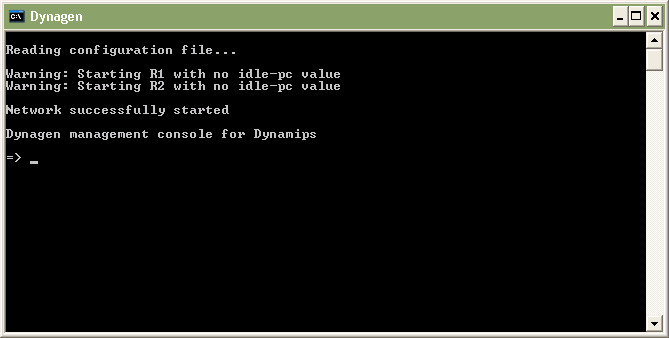
\includegraphics[width=0.75\textwidth]{dynamips_dynagen}
    \caption{Nástroj Dynagen spustený v prostredí Windows} \cite{obr_dynamips_dynagen}
    \label{obr:dynamips_dynagen}
\end{figure}

\subsection{WEB-IOU}

WEB-IOU je simulačný nástroj pre platformu Linux, ktorý podporuje výlučne Cisco IOU platformu. Jeho hlavnou výhodou je podpora Cisco prepínačov, ktorá pri Dynamips/Dynagen chýba. Jeho autorom je Andrea Dainese \cite{webiou_github, webiou_unetlab_unetlabv2}.Nástroj je v prevažnej mierie napísaný v jazykoch PHP a JavaScript \cite{webiou_github}. Podporuje iba výlučne vybrané Cisco smerovače na platforme IOU - IOS on Unix \cite{webiou_firewall_cx}. Je vhodný na trénovanie pri certifikáciách CCNP a do istej miery aj CCIE. 

Spravuje sa cez príkazový riadok. Používateľovi je dostupné web rozhranie. Portové čísla na vzdialený prístup sa zariadeniam prideľujú automaticky. Vzdialený prístup k zariadeniam v topológii je realizovaný protokolom \emph{telnet}. Na vytváranie topológii sa používa jednoduchý značkovací jazyk \emph{NETMAP}. Topológie môže ktokoľvek, kto má prístup k web rozhraniu, pretože ani tento nástroj nevie rozlišovať rôzne typy používateľov. Počet topológii, ktoré môžu byť súčasne spustené je obmedzené iba výkonom servera. Napriek tomu môžu na jednej topológii môžu pracovať aj viacerí študenti rovnakým spôsobom, ako pri nástroji Dynamips/Dynalab. Nástroj WEB-IOU tiež umožňuje prepojiť topológiu so živou sieťou \cite{webiou_real_network}. 

V súčasnosti sa už nástroj nevyvíja. Na obrázku \ref{obr:webiou} je znázornené webové rozhranie nástroja WEB-IOU.

\begin{figure}
    \centering
    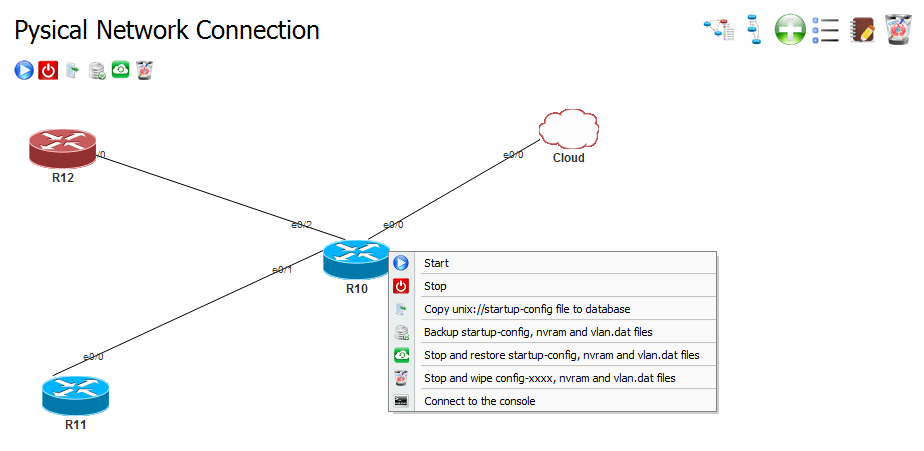
\includegraphics[width=0.75\textwidth]{webiou}
    \caption{Nástroj Dynagen spustený v prostredí Windows} \cite{obr_webiou}
    \label{obr:webiou}
\end{figure}

\subsection{Cisco VIRL}

VIRL, Virtual Internet Routing Lab, je komerčný simulačný nástroj sietí vyvíjaný spoločnosťou Cisco. Podporuje nielen Cisco smerovače a prepínače, ale aj zariadenia iných výrobcov, hoci ich integrácia nemusí byť jednoduchá. Výhodou oproti iným nástrojom je možnosť pridať podporované zariadenia do topológie ako LXC kontajner. Nevýhodou je, že nepodporuje Dynamips/Dynagen emuláciu, takže na ňom nie je možné využiť existujúce virtuálne zariadenia na katedre. Nástroj je postavený na platforme Linux (Debian) a je dostupný ako virtuálny stroj pre rôzne platformy. Je vhodný na trénovanie pri certifikáciách CCNP a do istej miery aj CCIE \cite{virl_cisco}. 

Spravuje sa cez príkazový riadok. Používateľovi je dostupné web rozhranie. Portové čísla na vzdialený prístup sa zariadeniam prideľujú automaticky \cite{virl_interfacett_1}. Vzdialený prístup k zariadeniam v topológii je realizovaný protokolmi \emph{telnet} a \emph{ssh}, po úprave aj \emph{vnc} \cite{virl_ciscoskills, virl_speaknetworks}. Na vytváranie topológii sa používa Nástroj \emph{VM Maestro}. Ten poskytuje možnosť, vopred si nakonfigurovať zariadenie podľa zvolených scenárov pomocou funkcie \emph{AutoNetkit}. Aj napriek tomu, že VIRL poskytuje pomerne podrobné možnosti na konfiguráciu zariadení a topológii, jeho používanie je pomerne obtiažne, hlavne pri vytváraní topológii \cite{virl_interfacett_1, virl_interfacett_2}. Cisco VIRL vie rozlišovať rôzne typy používateľov \cite{virl_cisco_features}. Počet topológii, ktoré môžu byť súčasne spustené je obmedzené iba výkonom servera. Napriek tomu môžu na jednej topológii môžu pracovať aj viacerí študenti rovnakým spôsobom, ako pri nástroji Dynamips/Dynalab \cite{virl_interfacett_2}. Nástroj tiež umožňuje prepojiť topológiu so živou sieťou \cite{virl_speaknetworks}. 

Nástroj v súčasnosti existuje iba vo verzii \emph{Personal Edition} s licenciou na 20 zariadení, čo výrazným spôsobom obmedzuje jeho využitie na katedre. V minulosti existovali aj verzie \emph{Personal Edition} s licenciou na 30 zariadení a \emph{Academic Edition}. Rozdiel medzi Personal a Academic Edition bol iba ten, že Academic Edition bol prístupný učiteľom a študentom za výhodnejšiu cenu. Podporované funkcionality boli zhodné v oboch verziách \cite{virl_edition_differences}. Na obrázkoch \ref{obr:virl_vmmaestro} a \ref{obr:virl_web} je znázornený nástroj na vytváranie topológii VM Maestro a webové rozhranie Cisco VIRL.

\begin{figure}
    \centering
    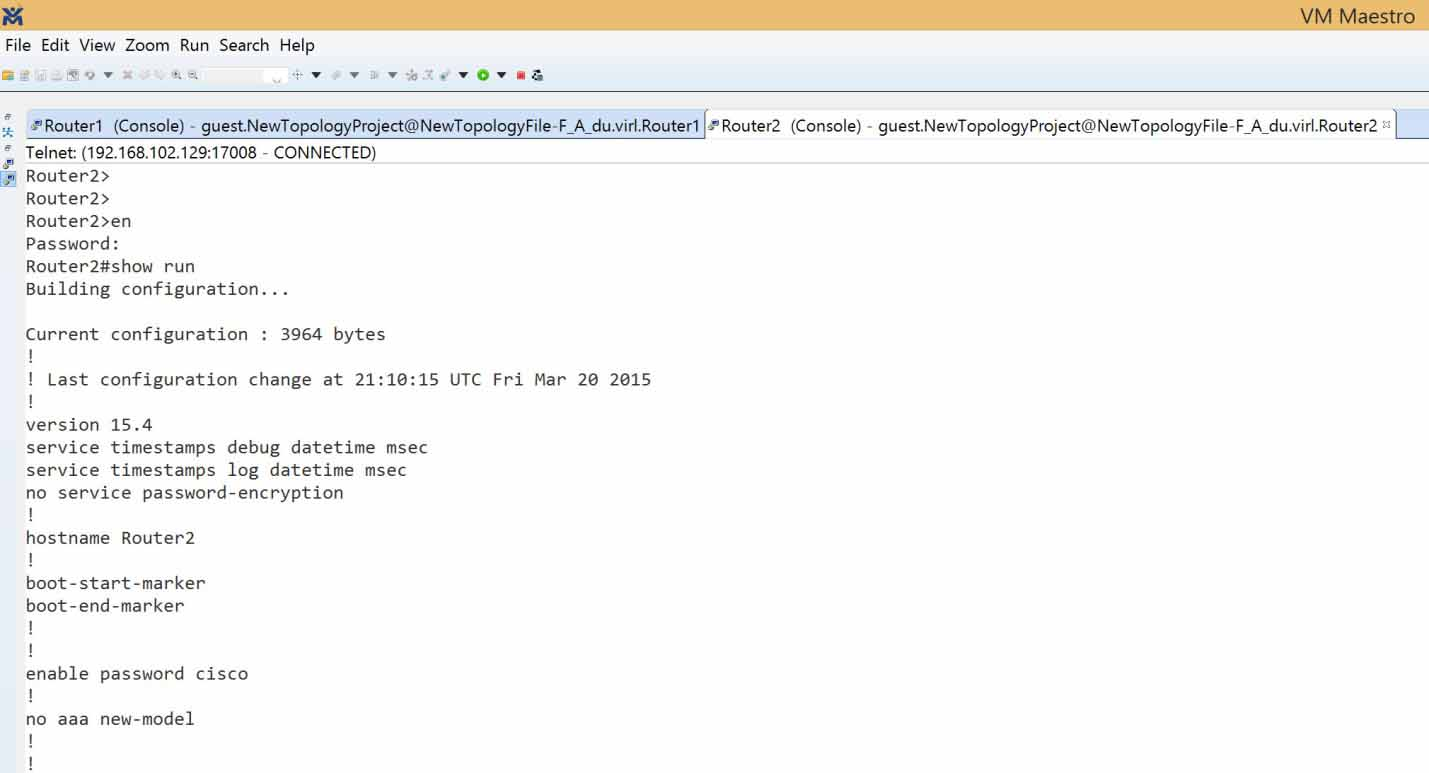
\includegraphics[width=0.75\textwidth]{virl_vmmaestro}
    \caption{VM Maestro} \cite{obr_virl_vmmaestro}
    \label{obr:virl_vmmaestro}
\end{figure}

\begin{figure}
    \centering
    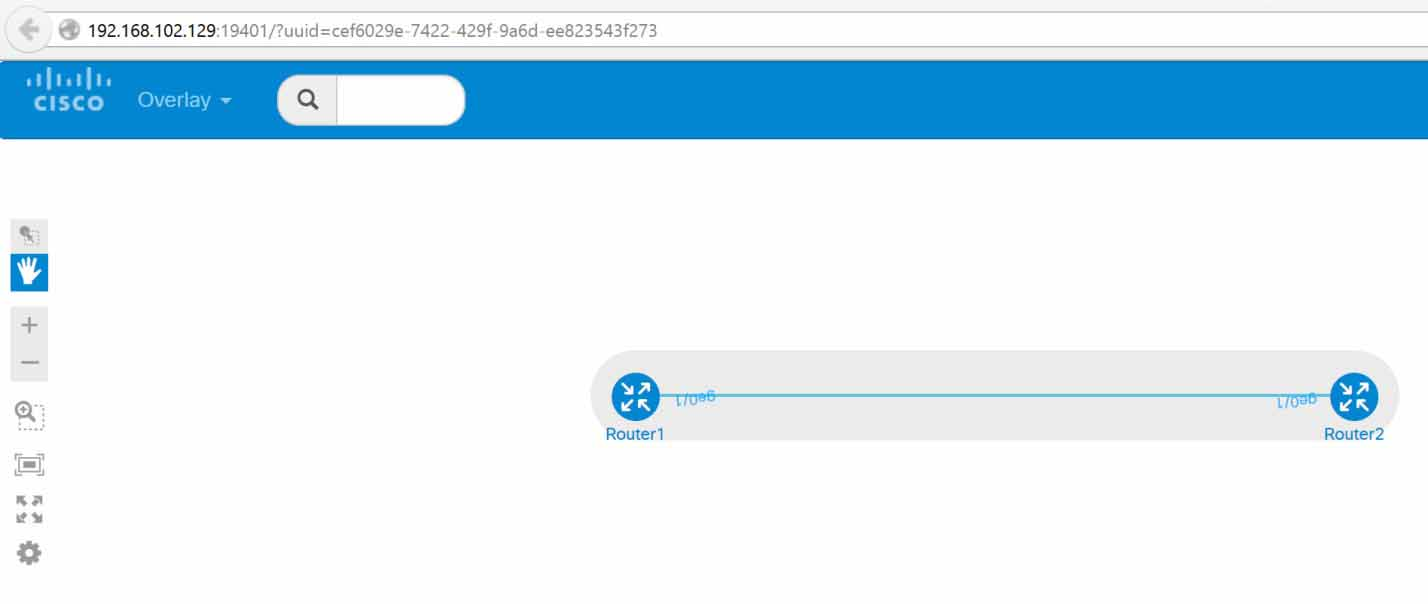
\includegraphics[width=0.75\textwidth]{virl_web}
    \caption{Cisco VIRL web rozhranie} \cite{obr_virl_web}
    \label{obr:virl_web}
\end{figure}

\subsection{VIRO}

VIRO je virtuálne laboratórium Ing. Petra Hadača. Nástroj vznikol ako výsledok jeho diplomovej práce. Jeho hlavnou výhodou je podpora Nokia smerovačov. Nástroj je na platforme Linux a využíva KVM. Nástroj podporuje aj smerovače ďalších výrobcov, pokiaľ podporujú beh v rámci QEMU/KVM. Ich podpora však nebola otestovaná. Nevýhodou je, že nepodporuje ani Dynamips, ani Cisco IOL zariadenia.

Spravuje sa prostredníctvom SSH. Používateľovi je dostupná VNC konzola. Portové čísla na vzdialený prístup sa zariadeniam prideľujú manuálne. Vzdialený prístup k zariadeniam v topológii je realizovaný ???. Na vytváranie topológii a správu zariadení sa používa grafický nástroj \emph{Virtual Machine Manager}. Na tento účel môžeme použiť aj nástroj \emph{virsh}, s ktorým grafický nástroj pracuje na pozadí. Topológie môže ktokoľvek, kto má prístup k SSH resp. VNC konzole, pretože nástroj VIRO nevie rozlišovať rôzne typy používateľov. Počet topológii, ktoré môžu byť súčasne spustené je obmedzené iba výkonom servera. Napriek tomu môžu na jednej topológii môžu pracovať aj viacerí študenti rovnakým spôsobom, ako pri nástroji Dynamips/Dynalab ???. Nástroj umožňuje prepojiť topológiu so živou sieťou, keďže KVM resp. virsh túto funkciu podporujú. Táto možnosť avšak nebola otestovaná ???. \cite{viro_hadac}.

V súčasnosti je nástroj pomerne funkčný, ale jeho vývoj doposiaľ nepokročil.

\subsection{UNetLab}

UNetLab, skrátene UNL, je simulačný nástroj pre platformu Linux, ktorý integruje všetky vyššie uvedené technológie najednom mieste: Dynamips, Cisco IOU aj zariadenia tretích strán (QEMU). Nástroj je postavený na platforme Linux. Jeho autorom je Andrea Dainese. V prevažnej mierie je napísaný v jazykoch PHP a JavaScript \cite{webiou_unetlab_unetlabv2, unetlab_github}. Je vhodný nielen na trénovanie pri Cisco certifikáciách, ale aj na testovanie kompatibility rôznych výrobcov.

Spravuje sa cez príkazový riadok. Používateľovi je dostupné web rozhranie. Portové čísla na vzdialený prístup sa zariadeniam prideľujú automaticky. Vzdialený prístup k zariadeniam v topológii je realizovaný protokolom \emph{telnet}. Topológie sa vytvárajú vo webovom rozhraní prepájaním uzlov medzi sebou pomocou myši. N sa používa jednoduchý značkovací jazyk \emph{NETMAP}. Topológie môže ktokoľvek, kto má prístup k web rozhraniu, pretože ani tento nástroj nevie rozlišovať rôzne typy používateľov, hoci v istej verzii nástroja táto funkcia bola podporovaná \cite{unetlab_github}. Počet topológii, ktoré môžu byť súčasne spustené je obmedzené iba výkonom servera. Napriek tomu môžu na jednej topológii môžu pracovať aj viacerí študenti rovnakým spôsobom, ako pri nástroji Dynamips/Dynalab. Jeden používateľ môže mať otvorenú práve jednu topológiu. Topológia sa dá zatvoriť až vtedy, keď v nej nie sú spustené žiadne zariadenia. Nástroj UNetLab tiež umožňuje prepojiť topológiu so živou sieťou pomocou \emph{bridge} rozhrania (pnet0) v topológii \cite{webiou_real_network}.

Vývoj tohto nástroja bol zastavený. UNetLab ďalej vyvíjala iná skupina vývojárov, ktorý nástroj premenovala na EVE-ng a migrovala ho z platformy Ubuntu 14.04 na Ubuntu 16.04. Jeho pôvodný autor následne začal s vývojom ďalšej verzie nástroja UNetLab, UNetLabv2. Na obrázku \ref{obr:unetlab_web} je znázornené webové rozhranie nástroja UNetLab.

\begin{figure}
    \centering
    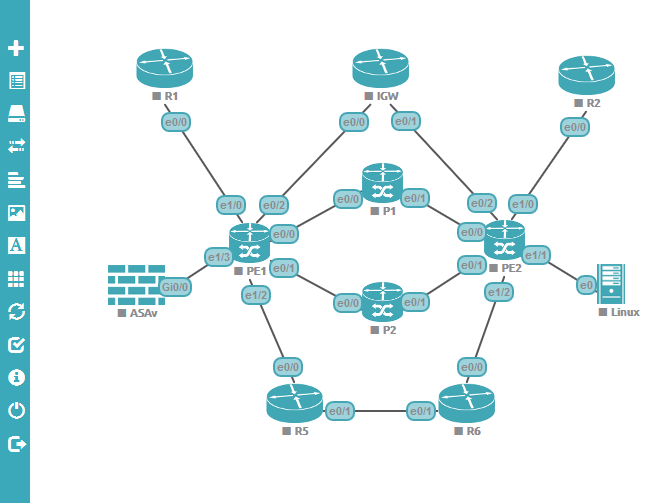
\includegraphics[width=0.75\textwidth]{unetlab_web}
    \caption{UNetLab web rozhranie}
    \cite{obr_unetlab_web}
    \label{obr:unetlab_web}
\end{figure}

\subsection{EVE-ng}

popis + rozdiely rôznych verzií (špeciálne pre EVE-ng) - PRIMÁRNE! + rozdiely vo funkcionalitách podľa tabuľky na oficiálnej stránke EVE-ng.

\subsection{GNS3}

- podporný nástroj pre tento projekt.

\subsection{UNetLabv2}

UNetLabv2 je nasledovníkom nástroja UNetLab. Je postavený na platforme Docker kontajnerov. Jednotlivé úlohy sú distribuované naprieč kontajnermi. To zaisťuje lepšiu škálovateľnosť pri zachovaní rovnakej funkcionality. Zatiaľ ešte nie je verejne nedostupný.

Architektúra nástroja UNetLabv2 je znázornená na obrázku \ref{obr:unetlabv2_arch}

\begin{figure}
    \centering
    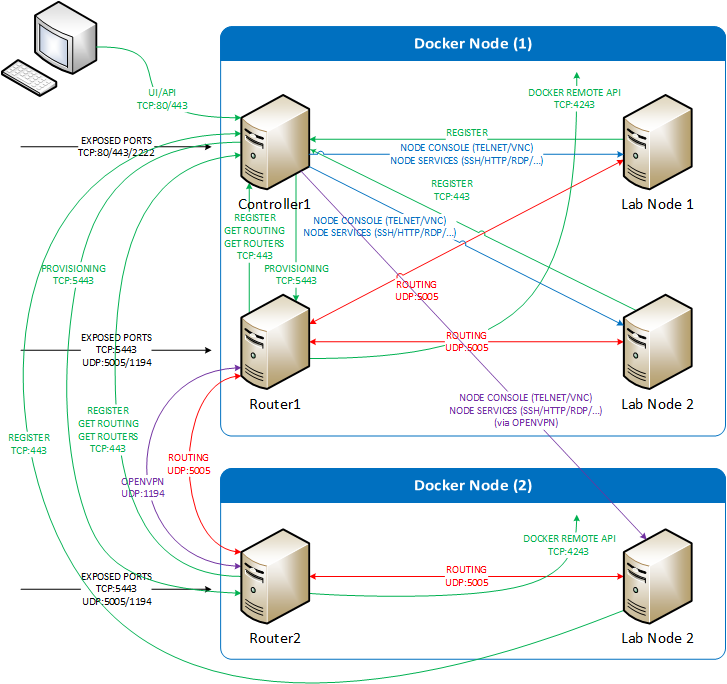
\includegraphics[width=0.75\textwidth]{unetlabv2_arch}
    \caption{Architektúra nástroja UNetLabv2} \cite{obr_unetlabv2_arch}
    \label{obr:unetlabv2_arch}
\end{figure}

\section{Vyhodnotenie}

Porovnanie GNS3 a EVE-ng.

Odôvodnenie, prečo som si vybral práve EVE-ng.